\documentclass[tikz,border=8pt]{standalone}
\usepackage{fontspec}
\usepackage{tikz}
\usetikzlibrary{arrows.meta,positioning}

\setmainfont[
  Path=C:/Windows/Fonts/,
  UprightFont=GOTHIC.TTF,
  BoldFont=GOTHICB.TTF,
  ItalicFont=GOTHICI.TTF,
  BoldItalicFont=GOTHICBI.TTF
]{Century Gothic}

\definecolor{navy}{HTML}{0C171F}

\tikzset{
  stage/.style={
    text=navy,
    font=\bfseries\fontsize{10.5}{13}\selectfont,
    align=center
  },
  label/.style={
    text=navy,
    font=\fontsize{10}{12.5}\selectfont,
    align=left,
    anchor=west
  },
  final/.style={
    draw=navy,
    line width=0.9pt,
    rounded corners=5pt,
    minimum width=5.5cm,
    minimum height=4.8cm,
    text=navy,
    align=center,
    font=\fontsize{10}{12.5}\selectfont,
    inner sep=14pt
  },
  arrow/.style={
    -{Latex[length=3mm,width=2mm]},
    draw=navy,
    line width=1pt
  }
}

\begin{document}
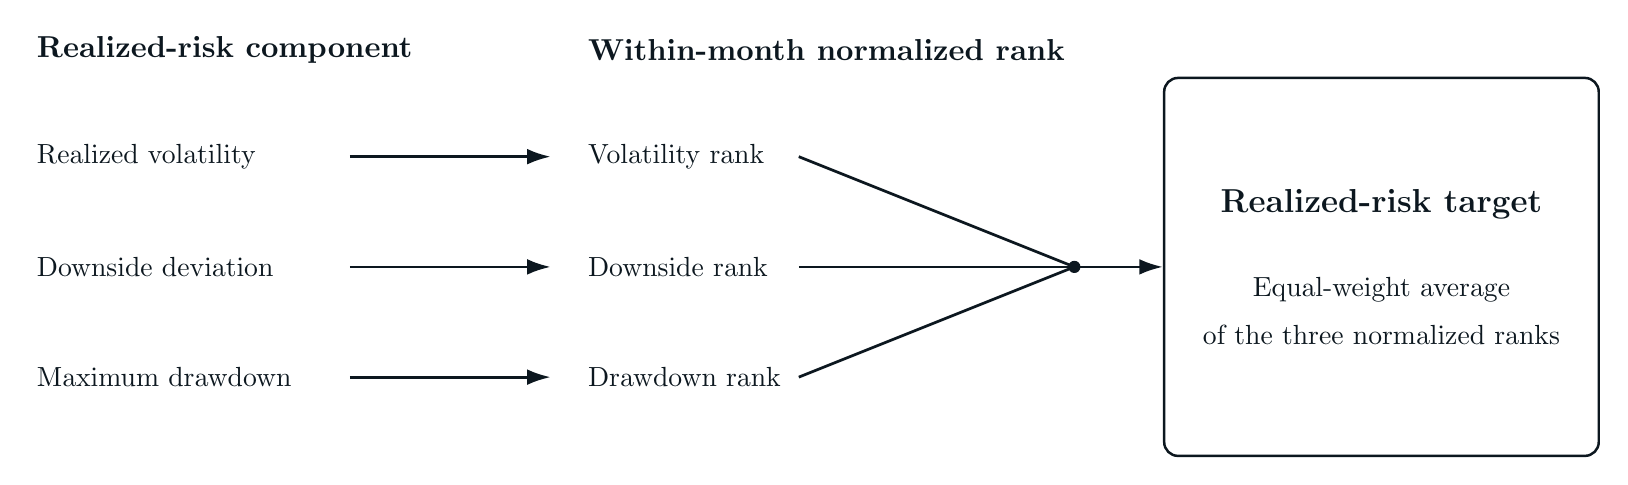
\begin{tikzpicture}
  \node[stage, anchor=west] at (0,0) {Realized-risk component};
  \node[stage, anchor=west] at (7.0,0) {Within-month normalized rank};

  \node[label] (vol) at (0,-1.35) {Realized volatility};
  \node[label] (down) at (0,-2.75) {Downside deviation};
  \node[label] (drawdown) at (0,-4.15) {Maximum drawdown};

  \node[label] (volrank) at (7.0,-1.35) {Volatility rank};
  \node[label] (downrank) at (7.0,-2.75) {Downside rank};
  \node[label] (drawrank) at (7.0,-4.15) {Drawdown rank};

  \node[final] (target) at (17.2,-2.75)
    {\textbf{\fontsize{12}{14}\selectfont Realized-risk target}\\[18pt]
     Equal-weight average\\[5pt]
     of the three normalized ranks};

  \coordinate (join) at (13.3,-2.75);

  \draw[arrow] ([xshift=4.1cm]vol.west) -- ([xshift=-0.35cm]volrank.west);
  \draw[arrow] ([xshift=4.1cm]down.west) -- ([xshift=-0.35cm]downrank.west);
  \draw[arrow] ([xshift=4.1cm]drawdown.west) -- ([xshift=-0.35cm]drawrank.west);

  \draw[navy, line width=1pt] ([xshift=2.8cm]volrank.west) -- (join);
  \draw[navy, line width=1pt] ([xshift=2.8cm]downrank.west) -- (join);
  \draw[navy, line width=1pt] ([xshift=2.8cm]drawrank.west) -- (join);
  \fill[navy] (join) circle (2.2pt);
  \draw[arrow] (join) -- (target.west);
\end{tikzpicture}
\end{document}
